\documentclass[11pt]{article}

% ====================================================
% PACKAGES
% ====================================================
\usepackage[margin=1in, headheight=13.6pt]{geometry}
\usepackage[T1]{fontenc}
\usepackage{lmodern}
\usepackage{microtype}
\usepackage{setspace}
\usepackage{tcolorbox}
\usepackage{amsmath, amssymb, mathtools}
\usepackage{siunitx}

\usepackage{graphicx}
\usepackage{float}
\usepackage{subcaption}

\usepackage{enumitem}
\usepackage{booktabs}
\usepackage{longtable}
\usepackage{array}
\usepackage{multirow}

\usepackage{xcolor}
\usepackage{hyperref}

\usepackage{fancyhdr}
\usepackage{lastpage}

\usepackage{listings}
\usepackage{indentfirst}
\usepackage[justification=centering]{caption}

% Python source style for \CodeListing
\lstdefinestyle{pystyle}{
    language=Python,
    basicstyle=\ttfamily\footnotesize,
    keywordstyle=\color{blue!60!black}\bfseries,
    stringstyle=\color{orange!70!black},
    commentstyle=\color{gray!60!black}\itshape,
    numbers=left,
    numberstyle=\tiny\color{gray!70},
    numbersep=8pt,
    breaklines=true,
    showstringspaces=false,
    frame=single,
    rulecolor=\color{gray!40},
    tabsize=4,
    columns=fullflexible,
    captionpos=b,
    literate={°}{{\textdegree}}1,
}
\lstset{style=pystyle}

\pagestyle{fancy}
\fancyhf{}
\lhead{\Assignment\ |\ \course}
\rhead{\Name\ |\ \today}
\cfoot{Page \thepage\ of~\pageref{LastPage}}

\hypersetup{
    colorlinks,
    linkcolor={red!50!black},
    citecolor={blue!50!black},
    urlcolor={blue!80!black}
}

\newcommand{\Name}{Arael Anaya}
\newcommand{\Assignment}{Homework 1}
\newcommand{\course}{Advanced Dynamics}

% Boxed final-answer environment
\newtcolorbox{result}{
    colback=blue!3!white,
    colframe=blue!40!black,
    boxrule=0.6pt,
    arc=2pt,
    left=6pt, right=6pt, top=4pt, bottom=4pt
}

% Code listing: sources the .py file directly.
\newcommand{\CodeListing}[3]{%
\IfFileExists{#1}%
    {\lstinputlisting[style=pystyle,caption={#2},label={#3}]{#1}}%
    {\begin{quote}\itshape Source file \texttt{#1} not found yet --- this
        listing will populate automatically once the file is written.\end{quote}}}

\begin{document}

% ====================================================
% PROBLEM 1
% ====================================================
\section*{Problem 1}

\begin{figure}[H]
    \centering
    
\includegraphics[width=0.95\linewidth]{Figures/Problem 1.png}
\end{figure}

\subsection*{Reference Frames}

\[
    \hat a_3=\hat n_3, \qquad \vec\omega^{A/N} = \dot\psi\,\hat a_3,
    \qquad \hat c_1=\hat a_1, \qquad \vec\omega^{C/A} = \dot\theta\,\hat a_1
\]
\[
    \vec\omega^{C/N} = \vec\omega^{A/N} + \vec\omega^{C/A} = \dot\theta\,\hat a_1 + \dot\psi\,\hat a_3
\]

\subsection*{Position of the Blade Center of Mass}

\[
    \vec r_{G/O} = d\,\hat a_1 + r\,\hat c_2,
    \qquad
    \begin{Bmatrix}\hat c_1\\ \hat c_2\\ \hat c_3\end{Bmatrix}
    =
    \underbrace{\begin{bmatrix}
        1 & 0 & 0\\
        0 & \cos\theta & \sin\theta\\
        0 & -\sin\theta & \cos\theta
    \end{bmatrix}}_{[R]^{A/C}}
    \begin{Bmatrix}\hat a_1\\ \hat a_2\\ \hat a_3\end{Bmatrix}
\]

\[
    \Rightarrow\qquad \vec r_{G/O} = d\,\hat a_1 + r\cos\theta\,\hat a_2 + r\sin\theta\,\hat a_3
\]

\subsection*{Velocity of $G$}

Applying the transport theorem between the $C$ and $N$ frames, with $\dfrac{{}^{C}d}{dt}\vec r_{G/O}=0$:
\[
    {}^{N}\vec v_G = \frac{{}^{C}d}{dt}\vec r_{G/O} + \vec\omega^{C/N}\times\vec r_{G/O}
    = \vec\omega^{C/N}\times\vec r_{G/O}
\]

\[
    {}^{N}\vec v_G =
    \begin{vmatrix}
        \hat a_1 & \hat a_2 & \hat a_3\\
        \dot\theta & 0 & \dot\psi\\
        d & r\cos\theta & r\sin\theta
    \end{vmatrix}
\]

Expanding the determinant:

\begin{align*}
    {}^{N}\vec v_G
    &= \big(0\cdot r\sin\theta - \dot\psi\, r\cos\theta\big)\hat a_1
     - \big(\dot\theta\, r\sin\theta - \dot\psi\, d\big)\hat a_2
     + \big(\dot\theta\, r\cos\theta - 0\cdot d\big)\hat a_3
\end{align*}

\begin{result}
\[
    {}^{N}\vec v_G =
    -r\dot\psi\cos\theta\;\hat a_1
    + \big(\dot\psi\, d - r\dot\theta\sin\theta\big)\hat a_2
    + r\dot\theta\cos\theta\;\hat a_3
\]
\end{result}

\subsection*{Acceleration of $G$}

Applying the transport theorem between the $A$ and $N$ frames, with $\vec\omega^{A/N} = \dot\psi\,\hat a_3$:
\[
    {}^{N}\vec a_G = \frac{{}^{A}d}{dt}\Big({}^{N}\vec v_G\Big) + \vec\omega^{A/N}\times {}^{N}\vec v_G
\]

\paragraph{Term I: $A$-frame derivative of $\vec v_G$.}
Differentiating each scalar component (treating $\hat a_1,\hat a_2,\hat a_3$ as constant):

\begin{align*}
    \frac{d}{dt}\big(-r\dot\psi\cos\theta\big)
        &= -r\ddot\psi\cos\theta + r\dot\psi\dot\theta\sin\theta \\
    \frac{d}{dt}\big(\dot\psi\, d - r\dot\theta\sin\theta\big)
        &= \ddot\psi\, d - r\ddot\theta\sin\theta - r\dot\theta^{2}\cos\theta \\
    \frac{d}{dt}\big(r\dot\theta\cos\theta\big)
        &= r\ddot\theta\cos\theta - r\dot\theta^{2}\sin\theta
\end{align*}

\[
    \frac{{}^{A}d}{dt}\big({}^{N}\vec v_G\big) =
    \big(r\dot\psi\dot\theta\sin\theta - r\ddot\psi\cos\theta\big)\hat a_1
    + \big(\ddot\psi\, d - r\dot\theta^{2}\cos\theta - r\ddot\theta\sin\theta\big)\hat a_2
    + \big(r\ddot\theta\cos\theta - r\dot\theta^{2}\sin\theta\big)\hat a_3
\]

\paragraph{Term II: $\vec\omega^{A/N}\times {}^{N}\vec v_G$.}
\[
    \vec\omega^{A/N}\times {}^{N}\vec v_G =
    \begin{vmatrix}
        \hat a_1 & \hat a_2 & \hat a_3\\
        0 & 0 & \dot\psi\\
        -r\dot\psi\cos\theta & \dot\psi\, d - r\dot\theta\sin\theta & r\dot\theta\cos\theta
    \end{vmatrix}
\]

\[
    \vec\omega^{A/N}\times {}^{N}\vec v_G =
    \big(r\dot\theta\dot\psi\sin\theta - d\dot\psi^{2}\big)\hat a_1
    - r\dot\psi^{2}\cos\theta\;\hat a_2
\]

\paragraph{Sum.} Adding the two terms component by component:

\begin{align*}
    \hat a_1: &\quad
        \big(-r\ddot\psi\cos\theta + r\dot\psi\dot\theta\sin\theta\big)
        + \big(r\dot\theta\dot\psi\sin\theta - d\dot\psi^{2}\big)
        = -d\dot\psi^{2} - r\ddot\psi\cos\theta + 2r\dot\theta\dot\psi\sin\theta \\[4pt]
    \hat a_2: &\quad
        \big(\ddot\psi\, d - r\dot\theta^{2}\cos\theta - r\ddot\theta\sin\theta\big)
        - r\dot\psi^{2}\cos\theta
        = d\ddot\psi - r\ddot\theta\sin\theta - r\big(\dot\theta^{2}+\dot\psi^{2}\big)\cos\theta \\[4pt]
    \hat a_3: &\quad
        r\ddot\theta\cos\theta - r\dot\theta^{2}\sin\theta
\end{align*}

\begin{result}
\begin{align*}
    {}^{N}\vec a_G =\;
    &\Big(-d\dot\psi^{2} - r\ddot\psi\cos\theta + 2r\dot\theta\dot\psi\sin\theta\Big)\hat a_1 \\
    +\;&\Big(d\ddot\psi - r\ddot\theta\sin\theta - r\big(\dot\theta^{2}+\dot\psi^{2}\big)\cos\theta\Big)\hat a_2 \\
    +\;&\Big(r\ddot\theta\cos\theta - r\dot\theta^{2}\sin\theta\Big)\hat a_3
\end{align*}
\end{result}

% ====================================================
% PROBLEM 2
% ====================================================
\newpage
\section*{Problem 2}

\begin{figure}[H]
    \centering
    
\includegraphics[width=0.95\linewidth]{Figures/Problem 2.png}
\end{figure}

\subsection*{Setup and Reference Frame}

In terms of the fixed basis $(\hat n_1,\hat n_2,\hat n_3)$,
\[
    \hat e_r =
    \begin{Bmatrix}
        \sin\phi\cos\theta\\
        \sin\phi\sin\theta\\
        -\cos\phi
    \end{Bmatrix},
    \qquad
    \hat e_\phi =
    \begin{Bmatrix}
        \cos\phi\cos\theta\\
        \cos\phi\sin\theta\\
        \sin\phi
    \end{Bmatrix},
    \qquad
    \hat e_\theta =
    \begin{Bmatrix}
        -\sin\theta\\
        \cos\theta\\
        0
    \end{Bmatrix}
\]

\subsection*{Derivatives of the Rotating Basis}

Differentiating each fixed-frame column vector and regrouping gives the kinematic identities

\[
    \dot{\hat e}_r = \dot\phi\,\hat e_\phi + \dot\theta\sin\phi\,\hat e_\theta,
    \qquad
    \dot{\hat e}_\phi = -\dot\phi\,\hat e_r + \dot\theta\cos\phi\,\hat e_\theta,
    \qquad
    \dot{\hat e}_\theta = -\dot\theta\sin\phi\,\hat e_r - \dot\theta\cos\phi\,\hat e_\phi
\]

\subsection*{Position, Velocity, and Acceleration}

With $\vec r_{m/O} = \ell\,\hat e_r$, differentiating once using $\dot{\hat e}_r$ gives the velocity,
\[
    {}^{N}\vec v_m = \ell\dot{\hat e}_r = \ell\big(\dot\phi\,\hat e_\phi + \dot\theta\sin\phi\,\hat e_\theta\big)
\]

Differentiating again, and using $\dot{\hat e}_\phi$ and $\dot{\hat e}_\theta$ to eliminate all derivatives of unit vectors,
\[
    {}^{N}\vec a_m = \ell\Big[
        \ddot\phi\,\hat e_\phi + \dot\phi\dot{\hat e}_\phi
        + \big(\ddot\theta\sin\phi + \dot\theta\dot\phi\cos\phi\big)\hat e_\theta
        + \dot\theta\sin\phi\,\dot{\hat e}_\theta
    \Big]
\]

Substituting $\dot{\hat e}_\phi = -\dot\phi\,\hat e_r + \dot\theta\cos\phi\,\hat e_\theta$ and $\dot{\hat e}_\theta = -\dot\theta\sin\phi\,\hat e_r - \dot\theta\cos\phi\,\hat e_\phi$ and collecting components:

\begin{align*}
    \hat e_r: &\quad -\dot\phi^{2} - \dot\theta^{2}\sin^{2}\phi \\
    \hat e_\theta: &\quad \ddot\theta\sin\phi + 2\dot\phi\dot\theta\cos\phi \\
    \hat e_\phi: &\quad \ddot\phi - \dot\theta^{2}\sin\phi\cos\phi
\end{align*}

\begin{result}
\[
    {}^{N}\vec a_m = \ell\Big[
        -\big(\dot\phi^{2}+\dot\theta^{2}\sin^{2}\phi\big)\hat e_r
        + \big(\ddot\theta\sin\phi + 2\dot\phi\dot\theta\cos\phi\big)\hat e_\theta
        + \big(\ddot\phi - \dot\theta^{2}\sin\phi\cos\phi\big)\hat e_\phi
    \Big]
\]
\end{result}

\subsection*{Equations of Motion (Newton's Second Law)}

The forces on the mass are the rod tension, directed along $-\hat e_r$, and gravity:
\[
    \vec F = -T\,\hat e_r - mg\,\hat n_3
\]

Solving the basis relations above for $\hat n_3$ gives
\[
    \hat n_3 = -\cos\phi\,\hat e_r + \sin\phi\,\hat e_\phi
\]

so that, in the rotating basis,
\[
    \vec F = \big(mg\cos\phi - T\big)\hat e_r - mg\sin\phi\,\hat e_\phi
\]

Applying $\vec F = m\,{}^{N}\vec a_m$ component by component:

\begin{align*}
    \hat e_r: &\quad mg\cos\phi - T = -m\ell\big(\dot\phi^{2}+\dot\theta^{2}\sin^{2}\phi\big) \\
    \hat e_\theta: &\quad 0 = m\ell\big(\ddot\theta\sin\phi + 2\dot\phi\dot\theta\cos\phi\big) \\
    \hat e_\phi: &\quad -mg\sin\phi = m\ell\big(\ddot\phi - \dot\theta^{2}\sin\phi\cos\phi\big)
\end{align*}

Solving each for the angular accelerations and the tension:

\begin{result}
\begin{align*}
    \ddot\phi &= \dot\theta^{2}\sin\phi\cos\phi - \frac{g}{\ell}\sin\phi \\[4pt]
    \ddot\theta &= -2\dot\phi\dot\theta\cot\phi \\[4pt]
    T &= mg\cos\phi + m\ell\big(\dot\phi^{2}+\dot\theta^{2}\sin^{2}\phi\big)
\end{align*}
\end{result}

% ====================================================
% PROBLEM 3
% ====================================================
\newpage
\section*{Problem 3}

\begin{figure}[H]
    \centering
    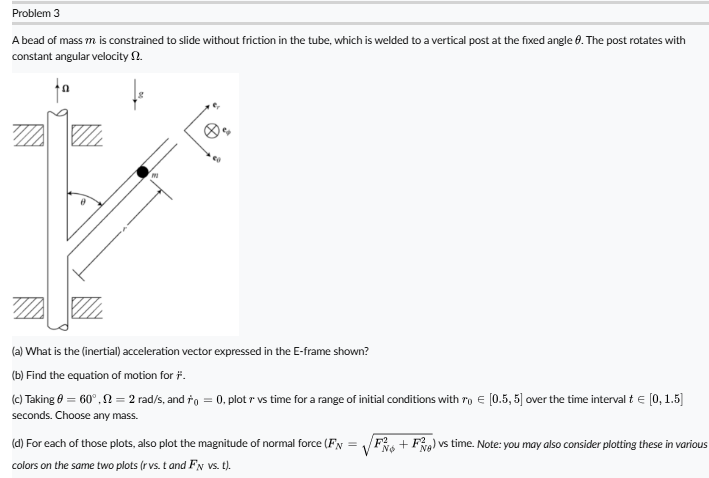
\includegraphics[width=0.95\linewidth]{Figures/Problem 3.png}
\end{figure}

\subsection*{Setup and Reference Frame}

The rotating tube frame $E$ has basis $(\hat e_r,\hat e_\theta,\hat e_\phi)$, with $\hat e_r$ along the tube axis. Since the tube makes a fixed angle $\theta$ with the post,
\[
    \hat n_3 = \cos\theta\,\hat e_r - \sin\theta\,\hat e_\theta,
    \qquad
    \vec\omega^{E/N} = \Omega\,\hat n_3 = \Omega\big(\cos\theta\,\hat e_r - \sin\theta\,\hat e_\theta\big)
\]

\subsection*{Velocity and Acceleration of the Bead}

The bead's position is $\vec r_m = r\,\hat e_r$. Applying the transport theorem,
\[
    {}^{N}\vec v_m = \frac{{}^{E}d}{dt}\vec r_m + \vec\omega^{E/N}\times\vec r_m
    = \dot r\,\hat e_r + \Omega r\big(\cos\theta\,\hat e_r - \sin\theta\,\hat e_\theta\big)\times\hat e_r
\]

Using $\hat e_r\times\hat e_r = 0$ and $\hat e_\theta\times\hat e_r = -\hat e_\phi$,
\[
    {}^{N}\vec v_m = \dot r\,\hat e_r + r\Omega\sin\theta\,\hat e_\phi
\]

Differentiating again,
\[
    {}^{N}\vec a_m = \frac{{}^{E}d}{dt}\big({}^{N}\vec v_m\big) + \vec\omega^{E/N}\times{}^{N}\vec v_m
    = \big(\ddot r\,\hat e_r + \dot r\Omega\sin\theta\,\hat e_\phi\big)
    + \Omega\big(\cos\theta\,\hat e_r - \sin\theta\,\hat e_\theta\big)\times\big(\dot r\,\hat e_r + r\Omega\sin\theta\,\hat e_\phi\big)
\]

Using $\hat e_r\times\hat e_\phi = -\hat e_\theta$, $\hat e_\theta\times\hat e_r = -\hat e_\phi$, $\hat e_\theta\times\hat e_\phi = \hat e_r$:
\[
    \vec\omega^{E/N}\times{}^{N}\vec v_m
    = -r\Omega^{2}\sin^{2}\theta\,\hat e_r - r\Omega^{2}\sin\theta\cos\theta\,\hat e_\theta + \dot r\Omega\sin\theta\,\hat e_\phi
\]

\begin{result}
\[
    {}^{N}\vec a_m =
    \big(\ddot r - r\Omega^{2}\sin^{2}\theta\big)\hat e_r
    - r\Omega^{2}\sin\theta\cos\theta\,\hat e_\theta
    + 2\dot r\Omega\sin\theta\,\hat e_\phi
\]
\end{result}

\subsection*{Equation of Motion (Newton's Second Law)}

The forces on the bead are gravity and the frictionless normal force of the tube wall (no $\hat e_r$ component):
\[
    \vec F = -mg\,\hat n_3 + F_{N\theta}\,\hat e_\theta + F_{N\phi}\,\hat e_\phi
    = \big(-mg\cos\theta\big)\hat e_r + \big(mg\sin\theta + F_{N\theta}\big)\hat e_\theta + F_{N\phi}\,\hat e_\phi
\]

Applying $\vec F = m\,{}^{N}\vec a_m$ component by component:
\begin{align*}
    \hat e_r: &\quad -mg\cos\theta = m\big(\ddot r - r\Omega^{2}\sin^{2}\theta\big) \\
    \hat e_\theta: &\quad mg\sin\theta + F_{N\theta} = -mr\Omega^{2}\sin\theta\cos\theta \\
    \hat e_\phi: &\quad F_{N\phi} = 2m\dot r\Omega\sin\theta
\end{align*}

\begin{result}
\[
    \ddot r = r\Omega^{2}\sin^{2}\theta - g\cos\theta
\]
\end{result}

and the normal-force components used in part (d),
\[
    F_{N\theta} = -m\big(g\sin\theta + \Omega^{2}r\sin\theta\cos\theta\big),
    \qquad
    F_{N\phi} = 2m\Omega\dot r\sin\theta,
    \qquad
    F_N = \sqrt{F_{N\theta}^{2} + F_{N\phi}^{2}}
\]

\subsection*{Numerical Implementation (Parts c--d)}

$\theta = 60^\circ$, $\Omega = 2\ \text{rad/s}$, $\dot r_0 = 0$, $r_0 \in [0.5,5]$.


\begin{figure}[H]
    \centering
    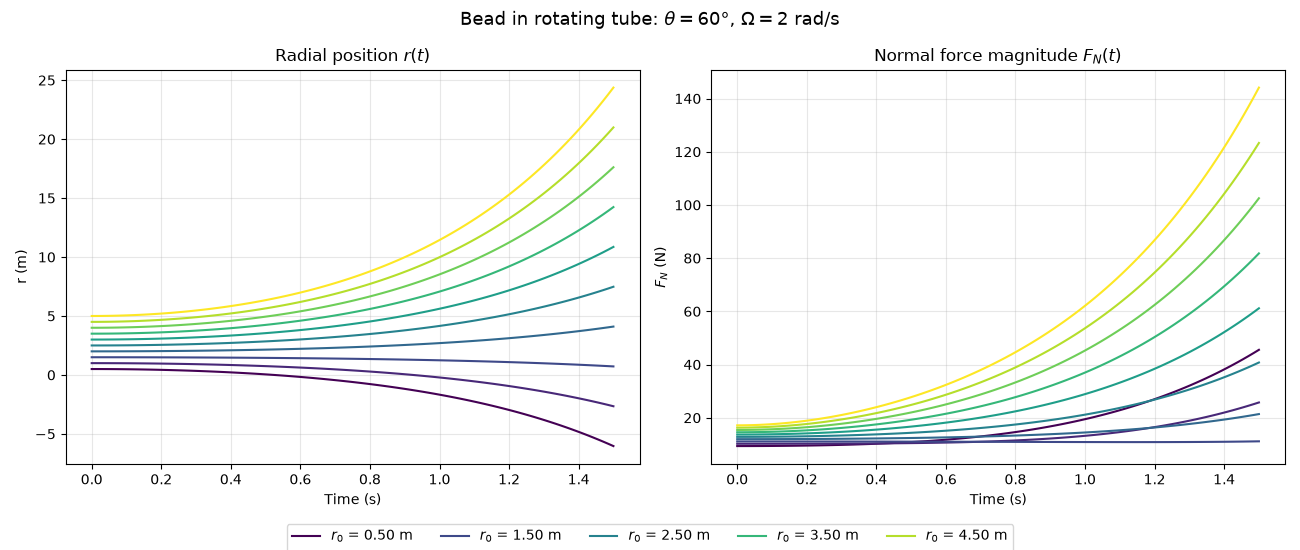
\includegraphics[width=0.95\linewidth]{Figures/Graphs/Problem 3 r and Fn vs t.png}
    \caption{Radial position $r(t)$ (part c) and normal-force magnitude $F_N(t)$ (part d) for $r_0\in[0.5,5]$, $\theta=60^\circ$, $\Omega=2\ \text{rad/s}$.}
    \label{fig:p3_r_FN_vs_t}
\end{figure}

% ====================================================
% PROBLEM 4
% ====================================================
\newpage
\section*{Problem 4}

\begin{figure}[H]
    \centering
    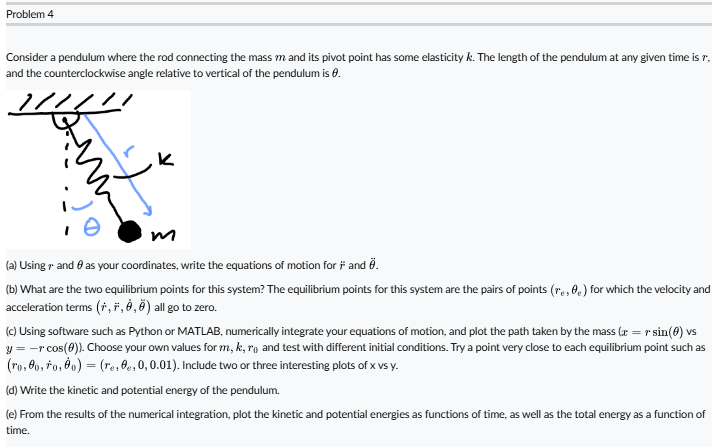
\includegraphics[width=0.95\linewidth]{Figures/Problem 4.png}
\end{figure}

\subsection*{Setup and Reference Frame}

The rotating frame $E$ has basis $(\hat e_r,\hat e_\theta)$, with $\hat e_r$ pointing from the pivot to the mass, so $\vec\omega^{E/N} = \dot\theta\,\hat n_3$, where $\hat n_3$ is the fixed out-of-plane axis. Since $\theta=0$ corresponds to the mass hanging straight down,
\[
    \hat n_{\text{down}} = \cos\theta\,\hat e_r - \sin\theta\,\hat e_\theta
\]

\subsection*{Velocity and Acceleration of the Mass}

With $\vec r_m = r\,\hat e_r$,
\[
    {}^{N}\vec v_m = \frac{{}^{E}d}{dt}\vec r_m + \vec\omega^{E/N}\times\vec r_m
    = \dot r\,\hat e_r + \dot\theta\,\hat n_3\times r\hat e_r
    = \dot r\,\hat e_r + r\dot\theta\,\hat e_\theta
\]

Differentiating again,
\[
    {}^{N}\vec a_m = \frac{{}^{E}d}{dt}\big({}^{N}\vec v_m\big) + \vec\omega^{E/N}\times{}^{N}\vec v_m
    = \big(\ddot r\,\hat e_r + \dot r\dot\theta\,\hat e_\theta + r\ddot\theta\,\hat e_\theta\big)
    + \dot\theta\,\hat n_3\times\big(\dot r\,\hat e_r + r\dot\theta\,\hat e_\theta\big)
\]

\[
    \dot\theta\,\hat n_3\times\big(\dot r\,\hat e_r + r\dot\theta\,\hat e_\theta\big) = \dot r\dot\theta\,\hat e_\theta - r\dot\theta^{2}\,\hat e_r
\]

\begin{result}
\[
    {}^{N}\vec a_m = \big(\ddot r - r\dot\theta^{2}\big)\hat e_r + \big(r\ddot\theta + 2\dot r\dot\theta\big)\hat e_\theta
\]
\end{result}

\subsection*{Part (a): Equations of Motion}

The forces on the mass are gravity and the spring tension $T = k(r-r_0)$ directed along $-\hat e_r$:
\[
    \vec F = -mg\,\hat n_{\text{down}} - T\,\hat e_r = \big(mg\cos\theta - T\big)\hat e_r - mg\sin\theta\,\hat e_\theta
\]

Applying $\vec F = m\,{}^{N}\vec a_m$ component by component:
\begin{align*}
    \hat e_r: &\quad mg\cos\theta - k(r-r_0) = m\big(\ddot r - r\dot\theta^{2}\big) \\
    \hat e_\theta: &\quad -mg\sin\theta = m\big(r\ddot\theta + 2\dot r\dot\theta\big)
\end{align*}

\begin{result}
\begin{align*}
    \ddot r &= r\dot\theta^{2} + g\cos\theta - \frac{k}{m}\big(r-r_0\big) \\[4pt]
    \ddot\theta &= -\frac{g\sin\theta + 2\dot r\dot\theta}{r}
\end{align*}
\end{result}

\subsection*{Part (b): Equilibrium Points}

Setting $\dot r=\ddot r=\dot\theta=\ddot\theta=0$ in the equations of motion:
\[
    0 = -\frac{g\sin\theta}{r} \;\Rightarrow\; \sin\theta = 0 \;\Rightarrow\; \theta_e = 0,\pi
\]
\[
    0 = g\cos\theta - \frac{k}{m}(r-r_0) \;\Rightarrow\; r = r_0 + \frac{mg}{k}\cos\theta
\]

\begin{result}
\[
    (r_e,\theta_e) = \left(r_0 + \frac{mg}{k},\; 0\right)
    \qquad\text{and}\qquad
    (r_e,\theta_e) = \left(r_0 - \frac{mg}{k},\; \pi\right)
\]
\end{result}

\subsection*{Numerical Implementation (Parts c, e)}

$m = 1\ \text{kg}$, $k = 10\ \text{N/m}$, $r_0 = 1\ \text{m}$, $\dot r_0 = 0$, $\dot\theta_0 = 0.01\ \text{rad/s}$ near each equilibrium $\theta_e = 0,\pi$; and $(r,\theta,\dot r,\dot\theta)_0 = (1,\,\pi/2,\,0.5,\,1)$ for a large swing away from equilibrium.

\subsection*{Part (c): Trajectory}

\begin{figure}[H]
    \centering
    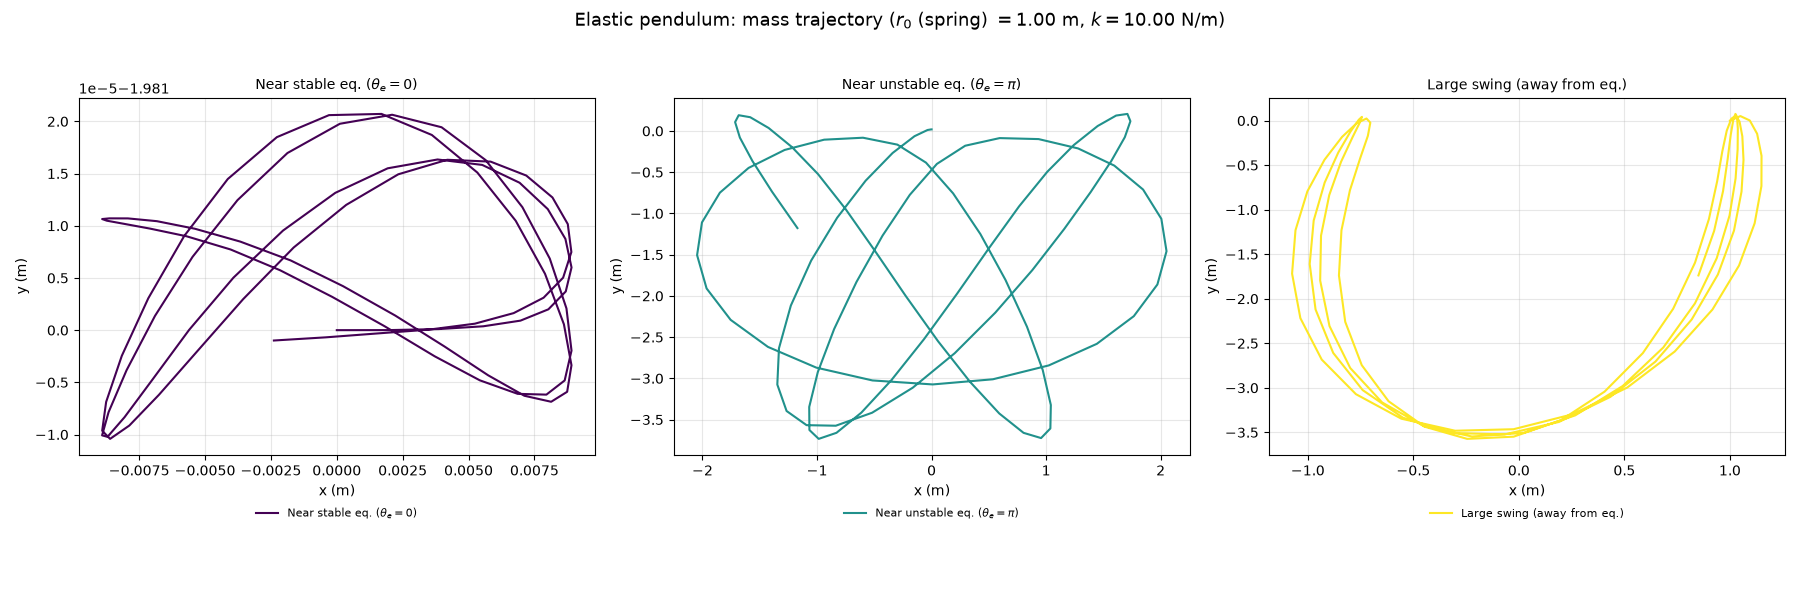
\includegraphics[width=\linewidth]{Figures/Graphs/Problem 4 x vs y.png}
    \caption{Trajectory $(x,y)$ near the stable equilibrium $(\theta_e=0)$, near the unstable equilibrium $(\theta_e=\pi)$, and for a large swing away from equilibrium.}
    \label{fig:p4_xy}
\end{figure}

\subsection*{Part (d): Kinetic and Potential Energy}

\[
    {}^{N}\vec v_m\cdot{}^{N}\vec v_m = \dot r^{2} + r^{2}\dot\theta^{2}
    \qquad\Longrightarrow\qquad
\]
\begin{result}
\[
    T = \frac12 m\big(\dot r^{2} + r^{2}\dot\theta^{2}\big)
\]
\end{result}

Taking the pivot as the reference height, with $y=-r\cos\theta$ and spring PE $\tfrac12 k(r-r_0)^2$,
\begin{result}
\[
    V = \frac12 k\big(r-r_0\big)^{2} - mgr\cos\theta
\]
\end{result}

\subsection*{Part (e): Energy vs.\ Time}

\begin{figure}[H]
    \centering
    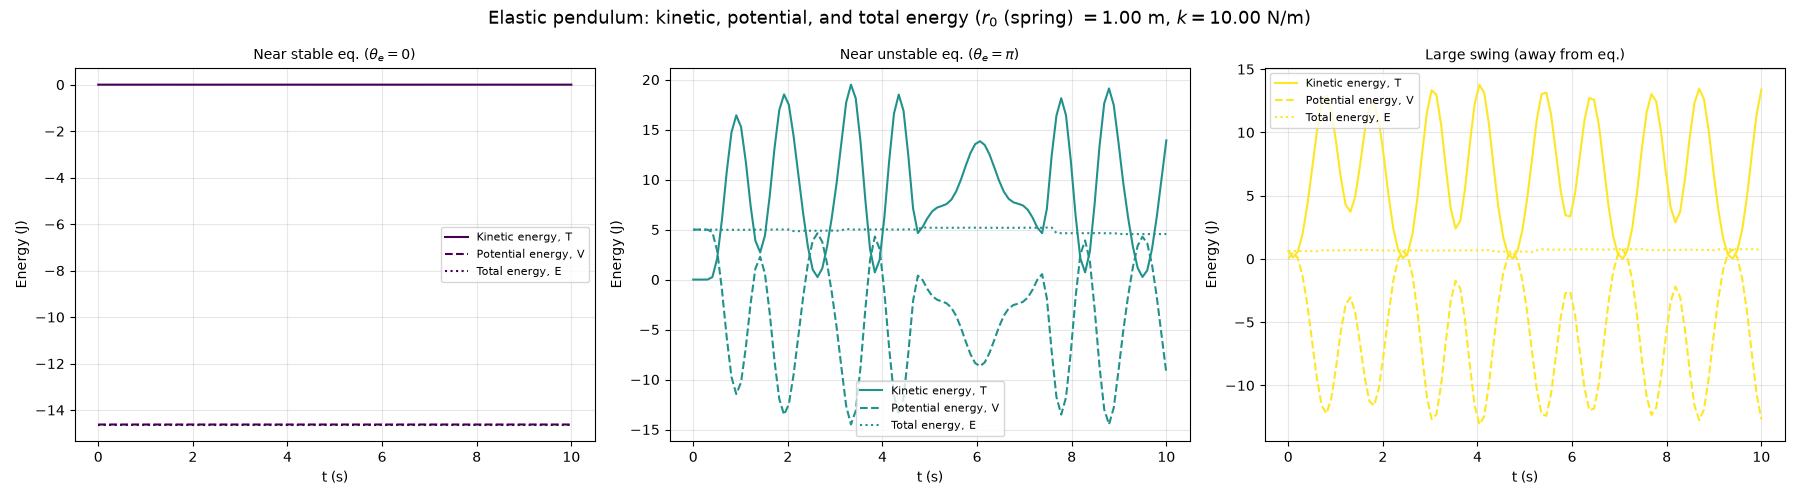
\includegraphics[width=\linewidth]{Figures/Graphs/Problem 4 Energy.png}
    \caption{Kinetic, potential, and total energy vs.\ time for each trajectory of Figure~\ref{fig:p4_xy}.}
    \label{fig:p4_energy}
\end{figure}

% ====================================================
% APPENDIX
% ====================================================
\newpage
\appendix
\section*{Appendix: Code Listings}

\subsection*{Problem 3 Code}
\CodeListing{../code/Problem3.py}{Numerical integration of the rotating-tube bead equation of motion and normal force.}{lst:p3}

\subsection*{Problem 4 Code}
\CodeListing{../code/Problem4.py}{Numerical integration of the elastic pendulum equations of motion, trajectory, and energy diagnostics.}{lst:p4}

\end{document}
